%remember to include in introduction:
%\begin{itemize}
%\item - define diffraction grating (transmission, reflection)
%\item - orders... energy dispersiveness of non n=0 orders
%\item - what is: diffraction efficiency
%\item - mention: in most cases of beamline design the grating eff is hardly considered, or left to the manufacturer. Even more rare to actually \textbf{test} the gratings for their actual efficiency.
%\end{itemize}

\chapter{Motivation: Why grating efficiency matters}

In 1821, when Joseph von Fraunhofer first resolved the sodium doublet lines using a diffraction grating he fashioned out of metal wire stretched between the grooves of two screws, he probably would not have anticipated the full scientific impact of his invention.
Immediately, these observations helped reinforce Fresnel's new wave theory of light \cite{Fra23}. % and Edinburgh Journal of Science, VII., VIII., 1827, 1828
More importantly, the diffraction grating quickly became the foundation of spectroscopy, superseding the prism as a wavelength-dispersive element with higher resolution, and applicable to radiation from the infrared to x-rays.  Eventually it would enable a huge range of experiments and new discoveries in all fields of science:
\begin{itemize}
\item In astronomy, Fraunhofer himself was the first to conduct spectroscopic measurements on light from the sun, moon, planets, and stars.  Shifts in the position of well-known absorption lines proved, using the Doppler Effect, that the universe was expanding.  Today, the composition and temperature of galactic objects is routinely measured using grating-based spectroscopic techniques.\footnote{In fact, the company that manufactured the gratings for this project also ruled the gratings used in the Hubble Space Telescope.}
\item In physics, visible spectroscopy of the hydrogen emission lines (Balmer Series) provided the data for Niels Bohr's explanation of electron levels in the atom.  Peter's discovery of the Zeeman Effect -- the splitting of emission lines in a magnetic field -- was accomplished using a 20-foot Rowland Circle spectrometer \cite{Zee97}; his results back up the modern version of quantum theory and the magnetic and spin quantum numbers.
\item In chemistry, many elements (such as caesium and rubidium, identified by Kirchhoff and Bunsen in 1860) were first discovered in trace amounts using spectral analysis.
\item Biologists and biochemists regularly use spectrophotometers to assay the concentration of a tagged reagent in a solution, making gratings a routine (and almost forgotten) tool in life sciences, pharmaceutical, and genetic research.
\end{itemize}

One common lamentation of the early spectroscopists was the faintness of the light leaving the grating; indeed, we can imagine them in darkened rooms, peering through telescope objectives,  straining to make out the faintest lines by eye:
% (Figure TODO):

\begin{quote}
\emph{Some lines can be distinguished in the spectrum of \emph{Procyon}; but they are seen with difficulty, and so indistinctly that their positions cannot be determined with certainty.  I \emph{think} I saw a line at the position D in the orange.}
\end{quote}
\begin{flushright}
Joseph Fraunhofer, in \emph{Prismatic and Diffraction Spectra} \cite[p.~61]{Fra98}
\end{flushright}

Photographic film -- and later, modern imaging devices like CCDs --  have probably succeeded in removing at least the physical pain associated with spectroscopy.  However, increases in grating efficiency are even more important and useful today as they would have been in 1830.  At visible wavelengths, more efficient gratings have already enabled a range of compact spectrometers with very high sensitivity, such as the convenient USB-powered computer peripheral in Figure \ref{1a}.  Other wavelength ranges are more challenging; grating efficiency is especially critical to the variety of soft x-ray spectroscopy experiments now taking place at synchrotrons around the world, where the low reflectivity of optical materials makes it difficult to build highly efficient devices.

\begin{figure}[htbp] %  figure placement: here, top, bottom, or page
   \centering
   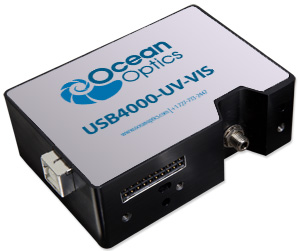
\includegraphics[scale=0.5]{../data/Chapter1/1a_oceanOptics/1a.jpg} 
   \caption{A rather sensitive, compact, visible light spectrometer (Ocean Optics USB4000-UV-VIS).  It uses a blazed reflection grating optimized for 300nm light, and connects to a personal computer using USB.  \textbf{Image credit: }\textsc{Ocean Optics, Inc.} \cite{Oce11}}
   \label{1a}
\end{figure}

Simply put, the \emph{diffraction grating efficiency} is the fraction of useful diffracted light outgoing from a grating, relative to the amount of incoming light.  (Chapter 3 offers a more formal definition.)  While spectroscopy experiments vary in hardware, instrumentation, and purpose, we can make a pair of very general observations on why the grating efficiency is so important.  From the point of view of an experimenter, it affects the amount of light available to their sample or detector, and therefore:
\begin{enumerate}
\item It affects the \emph{speed} at which experiments can be done, by determining the exposure time required to record data of sufficient quality.  In general, improvements in grating efficiency could reduce the amount of time for a given measurement -- or equivalently, increase the number of measurements that could be taken in a certain time period.  (For example, it takes anywhere from 3 minutes to several hours to measure a soft x-ray emission spectrum on the 8.0.1 beamline at the Advanced Light Source, depending on the concentration of the sample and the desired resolution.  One could argue that a factor of 2 optimization in the grating efficiency could almost double the number of users or the scientific throughput of the beamline.)
\item It affects the \emph{feasibility} of doing an experiment in the first place.  In situations where the experimental light source is extremely weak (for example, spectral analysis of faint stars in astronomy, or emission line measurements of trace elements in material science) the grating efficiency must be sufficient to raise the signal level above the background noise level seen by the detector.  This is no longer a question of patience; if the signal level is below the background noise, our unhappy experimentalist could accumulate detector readings all day (or indefinitely) to no avail.\footnote{In fact, Zeeman mentions in the introduction to his paper that he was inspired by Faraday, who spent the last years of his life trying, ``but in vain, to detect any change in the lines of the spectrum of a flame when the flame was acted on by a powerful magnet''.  Zeeman decided ``it might be yet worth while to try the experiment again with the excellent auxiliaries of the spectroscopy of the present time...'' \cite{Zee97}, brought on by Henry Rowland's new mechanically-ruled reflection gratings.}
\end{enumerate}

The motivation for this project was therefore to understand the factors affecting the efficiency of diffraction gratings, and to apply this knowledge to their optimization.  To accomplish this, we sought the ability to model gratings numerically and calculate their efficiency -- a useful outcome for all grating spectroscopy applications.  

However, we had another specific, selfish goal, which was actually our primary objective.  At the onset of this project, we were involved in the optical design of a soft x-ray emission spectrometer, destined for use on the REIXS beamline at the Canadian Light Source.  Working with David Muir, whose studies on spectrometer resolution are published in his M.Sc. thesis \cite{Mui06}, we attempted to simultaneously achieve both \emph{world-class resolution} and \emph{record efficiency} for this machine.\footnote{As it turns out, these two goals are implicitly in conflict; see Section \ref{resolutionGoals}.}  Therefore, although the calculation techniques presented in this thesis are general, our examination of trends in diffraction efficiency looks most closely at the types of gratings used in the soft x-ray regime.

Given our specific motivation, the following sections explain the ultimate goal of such a machine, and show how gratings are typically employed in soft x-ray spectroscopy.

\section{Soft X-ray Spectroscopy Techniques}
Soft x-rays are photons with energies in the range of approximately 100 to 10 000 eV (or wavelengths of about 10 to 0.1 nm).  Unlike with hard x-rays, which are highly penetrating, soft x-ray energies correspond to the binding energies of core-level electrons in common, lightweight elements.  This property is ironically responsible for both the experimental challenge of working with them -- they are quickly absorbed by any matter over very short distances -- as well as their inherent usefulness as a probe of the electronic structure in materials.

Soft x-ray experiments use this light -- usually created by a tuneable source such as a synchrotron -- and focus it onto a sample to be studied.  Two techniques provide complementary information: absorption spectroscopy, and emission spectroscopy.

\subsection{Absorption spectroscopy}
Absorption spectroscopy measures the absorption rate of photons as a function of their wavelength (or energy).  Experimentally, this is done by shining a monochromatic beam of light onto the sample and measuring the amount of light absorbed as the energy of the beam is changed.  

Figure \ref{1i} shows the available absorption processes, on the left side in red.  When the photon energy increases to become sufficient to excite an electronic transition in the material, dramatically more photons will be absorbed; this is known as an \emph{absorption edge}.  Near the edge, as photons are absorbed by exciting electrons from the core level into unoccupied levels, adjacent unoccupied  levels will have different probabilities of experiencing a transition, according to the quantum mechanical nature of the bonding in the material.  (Note that according to the selection rule for dipole radiation, only electron transitions with a change in orbital angular momentum quantum number $\Delta l = \pm 1$ are allowed, since momentum must be conserved and photons have an angular momentum [spin] of one unit.)  The absorption will increase for energies where the transition probability is higher; therefore, the absorption spectrum is actually a measure of the \emph{density of unoccupied states} for electrons in the material.\footnote{To be accurate, we should say the `\emph{partial} density of unoccupied states', since the vacancy left behind in the original electron state (``core-hole'') will affect the energy of the unoccupied states.}

\begin{figure}[htb] %  figure placement: here, top, bottom, or page
   \centering
   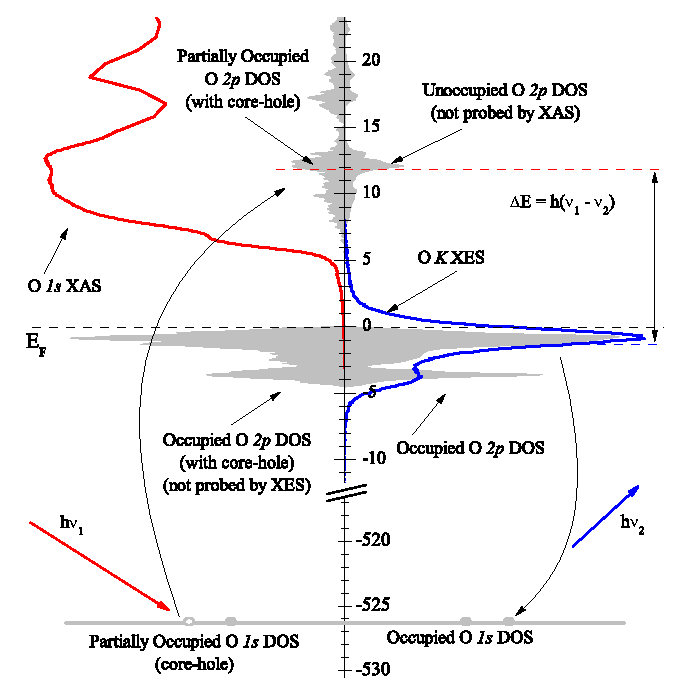
\includegraphics[scale=0.8]{../data/Chapter1/1i_sxsProcesses/1i.pdf} 
   \caption{X-ray absorption spectroscopy (on the left, in red) probes the density of \emph{unoccupied} electronic states, modified by the presence of a core-hole: a vacancy left behind by the excited electron.  In this example for oxygen, the absorption edge starts at 6 eV above the Fermi level, labelled $E_F$.\\X-ray emission spectroscopy (on the right, in blue) probes the density of \emph{occupied} valence states, as a valence electron decays by emitting a photon to fill the core-hole.  In this diagram, the absorption and emission spectrum have been plotted vertically to line up with the schematic of the energy levels; they are conventionally plotted on a horizontal energy axis.  Grey areas represent the computed density of states.  \textbf{Image from: }Ref. \cite{McL10}}
   \label{1i}
\end{figure}

One outstanding question concerns how the absorption rate is measured -- how do we know how many photons were absorbed?  Perfect absorption spectroscopy would shine the beam clear through the sample, and measure the intensity of the beam before and after to determine the fraction of light absorbed.  While \emph{transmission measurements} like this are feasible with hard x-rays, the short attenuation length of soft x-rays would require prohibitively thin samples for any beam to be left on the other side.  Instead, different measurements are used as a proxy for the total absorption rate:
\subsubsection{Total Electron Yield}
For the excited electron, the most probable decay mechanism is to quickly relax into a lower-energy state, transferring its energy to a more loosely bound electron in the process.  This secondary electron, known as an Auger electron, can then be ejected from the sample -- assuming it is close enough to the surface.  The \textbf{total electron yield} (TEY) method determines the absorption rate by measuring the electric current that must flow into the sample to neutralize the ejected electrons and keep the sample uncharged.  (Experimentally, this is done by simply connecting a wire to the sample holder, and placing a sensitive ammeter along the path to a solid ground connection.)

TEY measurements are difficult for some samples, either because an insulating sample doesn't allow current to flow in to replenish the ejected electrons (``sample charging''), or because electrons ejected deep in the material are reabsorbed elsewhere.  This makes TEY measurements most sensitive to absorption events near the surface ($\sim$2nm), and restricts them to conductive samples.
\subsubsection{Total Fluorescence Yield}
Total Fluorescence Yield (TFY) measurements overcome these problems by using a light-sensitive detector near the sample.  Although several orders of magnitude less probable than the Auger decay process, excited states can also relax by emission of a photon.  Instead of ejected electrons, TFY measures the intensity of all photons emitted during the decay, which makes it applicable to both insulating and non-insulating samples.  Because photons have a greater escape depth than electrons, this technique is also able to probe deeper within a material than TEY can.  Due to the low probability of fluorescence transitions compared to Auger transitions (several orders of magnitude), TFY measurements benefit greatly from concentrated samples and a light source which is capable of high intensity.

\subsection{Emission spectroscopy}
While absorption measurements provide information about the \emph{unoccupied} states, we can also study what happens \emph{after} the initial photon is absorbed.  When a core-level electron is promoted by the absorption of a photon, it leaves behind a ``core-hole'', and the atom (or molecule, or crystal) is left in an excited state.  While there are many ways for the system to collapse back to the ground state, there is a small probability that some valence-band electron will decay to fill the core-hole by the emission of another photon.  Since the energy of the emitted photon will match the energy difference between that valence electron and the core level, the intensity distribution of \emph{all emitted light} will correspond to the probability of finding electrons in the valence band at those energies.  Therefore, if we could collect the \emph{fluorescence} emitted from the sample and plot its intensity as a function of energy, we would have a measure of the \emph{density of occupied states} for electrons in the material.  In this way, emission spectroscopy provides information on the bound electronic states, which is not present in the absorption spectrum.

Experimentally, XES measurements are done by illuminating the sample with a fixed photon energy above the absorption edge.  The fluorescence is captured using an energy- (or wavelength-)sensitive detector which is tuned to the energy range just below the absorption edge.  Over time, an intensity spectrum is built up from the collected photons (Figure \ref{1i}, Figure \ref{1e}).  Since fluorescence transitions are a random process, and highly improbable compared to other decay mechanisms like Auger decay, XES measurements require a sufficient exposure time to build up good statistics.  They also benefit greatly from a high-intensity beam source and an efficient detector -- such as a sensitive spectrometer with high-efficiency gratings.

\subsubsection{Resonant Inelastic X-ray Scattering (RIXS)}
An advanced form of XES is known as RIXS (\emph{Resonant Inelastic X-ray Scattering}).  Instead of exciting a sample with a photon energy well above the absorption edge, the energy of the beam is tuned to match transitions previously identified in the absorption spectrum (or stepped incrementally through this range).  This allows the experimenter to preferentially excite into specific electronic states: at \emph{resonance}, the transition probability will be extremely high because the exciting photon energy exactly matches the transition energy and the emitted photon energy.

RIXS is a one-step process, but it can be explained mathematically as a simultaneous two-step process which combines absorption and emission: from the initial electronic state, an incoming photon is absorbed, creating a ``core-hole'' and an excited electronic configuration.  This intermediate state decays by the emission of another photon into a final state, and this transition doesn't necessarily need to involve the original electron.  The difference in energy of the emitted and incident photons provides an \emph{energy-loss spectrum} describing the nature of excitations within the material.

According to this two-step explanation, RIXS can probe transitions that would be forbidden by the dipole selection rule. For example, a 2p electron could be excited into a 3d state, and another 3d electron with a slightly different energy could collapse to fill the 2p hole, thereby effectively creating of a `d-d' excitation \cite{But96}.
\subsection{Importance of Soft X-ray Spectroscopy (SXS)}
Soft x-ray spectroscopy is a valuable tool in material science for its ability to gain insight into the electron environment within a material.  Since the electronic structure determines the bonding between atoms and thereby a material's mechanical, chemical, and physical properties, this is a big deal indeed.  Additionally, x-ray spectroscopy has a few complementary advantages over other analytical techniques like neutron diffraction and photoemission spectroscopy:
\begin{itemize}
\item It is \textbf{element-specific}: for a material containing a number of elements, it is usually possible to find absorption edges for each element that do not overlap with the others, making it possible to independently probe the bonding environment of each.  For example, in an organic sample containing carbon, nitrogen, and oxygen, one can  probe the oxygen using the O 1s absorption at 543 eV, and then separately excite the nitrogen 1s electrons at 410 eV.
\item More than being just element-specific, it is also \textbf{site-specific}: soft x-ray spectra make it possible to distinguish, for example, single-bonded carbon atoms at one location in a molecule from double-bonded atoms at another.
\item Depending on the detection technique, it can be \textbf{surface-sensitive} or \textbf{bulk-sensitive} (i.e.: it can probe through surface contamination or oxidation, testing the nature of the material below).
\end{itemize}

Additionally, there are a few experimental considerations which make SXS desirable:
\begin{itemize}
\item It can be done \textbf{non-destructively} on whole samples, without having to crush them into powders, dilute them in solution, etc.  It can also allow in-situ measurements of samples created directly within the vacuum chamber -- for example, crystal samples created using sputtering or vapour deposition techniques.
\item Because of the high brightness and small size of synchrotron beams, it can be done on \textbf{very small and thin samples}.  Since the penetration depth of soft x-rays is so short, the interaction volume created by the beam will be tiny regardless of the sample thickness, making it a very useful characterization technique for thin film samples and even monolayers.
\end{itemize}
One obvious experimental disadvantage is that these techniques require access to synchrotron accelerators to produce the soft x-ray beam, which -- for the foreseeable future -- are not yet available in convenient desktop or bench-top models.  Additionally, since soft x-ray experiments must be performed under ultra-high vacuum (UHV) conditions (see section \ref{challengesSXS}), samples must either be UHV-compatible or carefully isolated from the vacuum environment behind thin windows.

Despite these limitations, SXS techniques have created some notable and very interesting discoveries in physics; some highlights are listed here:
\begin{itemize}
\item In 1990, de Groot et. al. presented the first comprehensive understanding of soft x-ray absorption in transition metal compounds.  Not only did they produce some state-of-the-art experimental spectra for the time, but they also gave a thorough interpretation of them using crystal field atomic-multiplet theory \cite{deG90}.

\item Butorin et. al. published the first RIXS studies of transition metals, and discovered \emph{d-d} excitations in manganese oxide \cite{But96}.

\item Recently, Braicovich et. al. used RIXS to measure the dispersion of magnetic excitations in cuprate superconductors.  This study also found a magnetic dispersion branch that had never been found before using neutron scattering, and found that these types of materials are in non-homogenous spin states, revealing a bit more about the mysterious nature of cuprate superconductors \cite{Bra10}.

\item With the proper experimental equipment, RIXS studies can also be done on gaseous samples.  In 2011, Pietzsch et. al. measured very high resolution RIXS on oxygen gas (O$_2$) to observe the vibronic structure.  The exciting result from this study was the presence of spatial quantum beats in their spectra -- essentially, an observation of quantum mechanical interference like the famous double-slit experiment, but using excitations into different states instead of transmission through different slits \cite{Pie11}.
\end{itemize}

\section{Spectroscopy Instrumentation}
The preceding sections make it clear that to perform soft x-ray spectroscopy experiments, we need three capabilities:
\begin{enumerate}
\item Obviously, one needs a source of soft x-rays -- typically, the brighter, the better.  This became possible with the advent of of synchrotron particle accelerator facilities, which emit broad-spectrum x-rays as relativistic electrons are forced to change their path by bending magnets.\footnote{Much more intense synchrotron light can be generated by ``insertion devices'' known as \emph{undulators} and \emph{wigglers}, in which an alternating array of magnets in a straight section of the accelerator forces the electron beam to bend many times over a distance of a few meters.  Although light from insertion devices still contains of a range of wavelengths, its spectrum consists of sharp intensity peaks which can be adjusted to the desired wavelength by changing the strength of the magnetic field.  We intentionally avoid going into too much detail on synchrotron physics in this thesis; more information can be found in Ref. \cite{Pea97}.}
\item \textbf{For absorption and emission spectroscopy:}\\
From this broad spectrum of light, one needs to produce a nearly monochromatic beam of light to shine onto the sample, and must be able to adjust the energy of this beam.  This is the role of a \emph{monochromator}, which takes a broad-spectrum light source and extracts a small range of wavelengths from it (Figure \ref{1b_monochromator}).
\item \textbf{Additionally, for emission spectroscopy:}\\
One must be able to capture the light emitted from the sample and resolve it by wavelength.  The end goal is to measure the relative intensity as a function of wavelength (or energy); this is accomplished using a \emph{spectrometer} (Figure \ref{1b_rowlandSpectrometer}).
\end{enumerate}

\begin{figure}[htbp] %  figure placement: here, top, bottom, or page
   \centering
   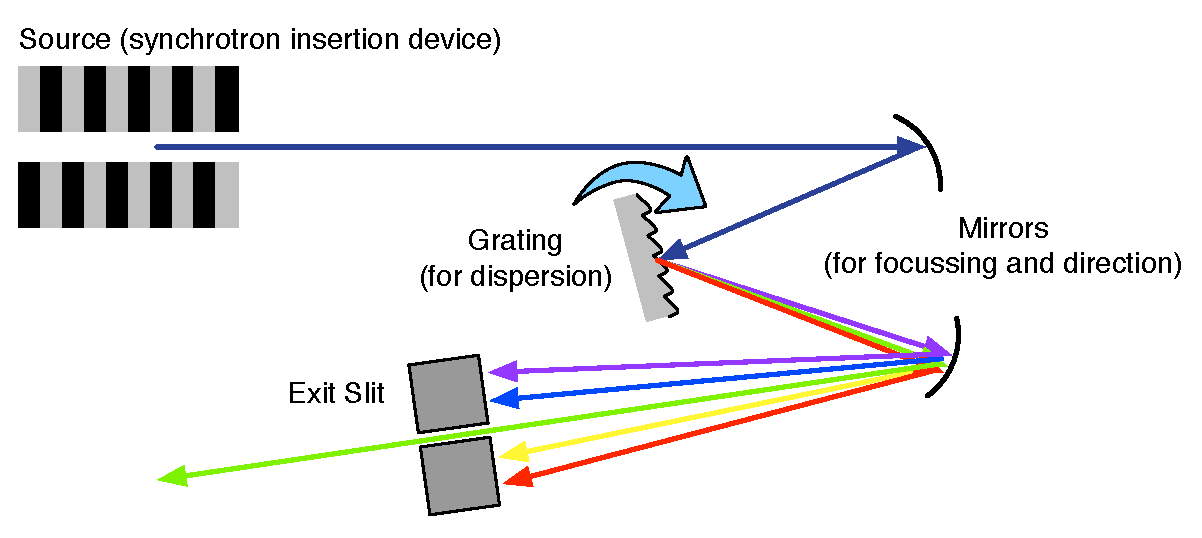
\includegraphics[scale=0.6]{../data/Chapter1/1b_spectrometerSchematic/1b_monochromator.pdf} 
   \caption{In this schematic of a grating monochromator, light from the source is focussed by mirrors and dispersed by the grating. An exit slit picks out the desired wavelength or energy range, and blocks the remaining light.  Depending on the design, the output wavelength can be adjusted by changing the angle of the grating, the angle of the mirrors, and/or the position of the exit slit.  (The resolution -- the energy bandwidth of the outgoing light -- depends on the dispersion of the grating, the geometry, and the size of the exit slit.  An ideal monochromator would produce truly monochromatic light, but this would require an infinitely small slit.)}
   \label{1b_monochromator}
\end{figure}

\begin{figure}[htbp] %  figure placement: here, top, bottom, or page
   \centering
   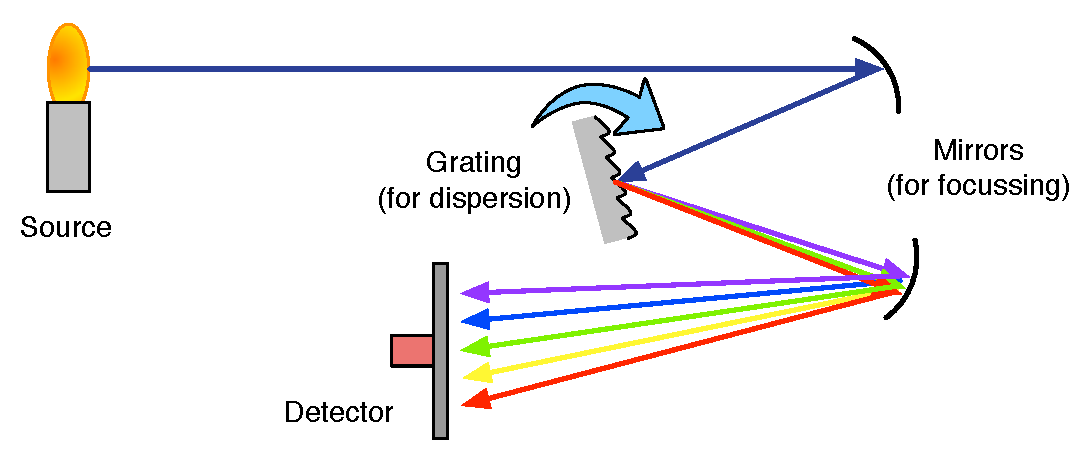
\includegraphics[scale=0.6]{../data/Chapter1/1b_spectrometerSchematic/1b_mirrorSpectrometer.pdf} 
   \caption{In this schematic of a grating spectrometer, mirrors are used to focus light from the source (or entrance slit) onto the detector, passing over a plane grating en-route to disperse the light by wavelength.  (This is a \emph{Czerny-Turner} arrangement, typical of compact visible-light designs like the one in Figure \ref{1a}.)  Since the grating diffracts different wavelengths at different angles, the intensity distribution across the detector surface creates a spectrum related to the wavelength (or photon energy).}
   \label{1b_mirrorSpectrometer}
\end{figure}

\begin{figure}[htbp] %  figure placement: here, top, bottom, or page
   \centering
   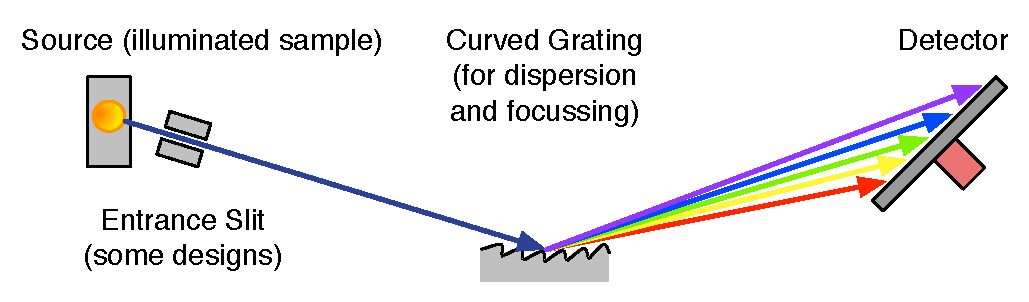
\includegraphics[scale=0.6]{../data/Chapter1/1b_spectrometerSchematic/1b_rowlandSpectrometer.pdf} 
   \caption{The spectrometer in this schematic uses a curved grating to both disperse light by wavelength, and focus it onto the detector.  (This is typical of soft x-ray designs where the poor reflectivity of additional mirrors is usually avoided.)  The intensity distribution along the surface of the detector can be converted into a spectrum with respect to wavelength or energy.  Since the detector only captures a limited range of outgoing angles, it can be moved to pick out the desired wavelength window for each measurement.}
   \label{1b_rowlandSpectrometer}
\end{figure}





\subsection{Beamline optics: Monochromators and Spectrometers}
\subsubsection{Monochromators}
The role of a monochromator (shown schematically in Figure \ref{1b_monochromator}) is to pick out a narrow range of wavelengths from a chromatic light source, and deliver the monochromatic beam to the experiment.  For infrared light out to soft x-rays, diffraction gratings provide the most efficient way of separating the incoming beam based on wavelength.\footnote{For hard x-rays, monochromators use ``natural'' diffraction gratings consisting of atomic planes in blocks of single crystals, since the inter-atomic spacing is comparable to the short wavelength of the light; these might be analyzed more appropriately using Bragg scattering theory than the electromagnetic approach we take for the man-made structures in this thesis.}  When the incidence angle and mounting angle of the grating are chosen to direct a single ($n\neq0$) diffraction order toward the exit slit, the wavelength term in the grating equation (equation \ref{gratingEquation})
\begin{eqnarray*}
n\lambda / d = \sin\theta_{2,n} - \sin\theta_{2}
\end{eqnarray*}
creates a dependence on the sine of the outgoing angle $\theta_{2,n}$, so that shorter wavelengths leave more normal, and longer wavelengths leave at more grazing angles.  Depending on the optical and mechanical design, the output wavelength can be selected by changing the angle of the grating, the angle of the mirrors (and hence the incidence angle onto the grating), and/or the position of the exit slit.

The resolution of the monochromator  -- ie: the bandwidth of wavelengths present in the output light -- depends on the angular dispersion of the grating, the geometry, and the size of the exit slit; an ideal device would obviously produce a perfectly monochromatic beam, but this would require an infinitely-small exit slit.  (In practice, the size of the exit slit is used to adjust the resolution, in an unavoidable trade-off against the amount of flux produced.)  Resolution is measured as the energy bandwidth $\Delta E$ (full width at half-maximum) for a given central energy; for example: $\Delta E = 500$ meV at 1000 eV.   Often it is more convenient to normalize it as the \emph{resolving power} $RP = E/\Delta E$, which has the benefit of being identical when measured in wavelength as well:
\begin{eqnarray}
RP = \frac{E}{\Delta E} = \frac{hc/\lambda}{\Delta \lambda \, \dif E/\dif \lambda} = \frac{hc/\lambda}{\Delta \lambda\, (-hc / \lambda^2)} =  \frac{\lambda}{-\Delta \lambda} \rightarrow \frac{\lambda}{\Delta \lambda}
\end{eqnarray}

In addition to dispersing the light by wavelength, monochromators must also act to \emph{focus} light from the source, typically onto the exit slit, or onto the focal point of a downstream mirror.  The schematic shown in Figure \ref{1b_monochromator} is a \emph{plane grating monochromator (PGM)}, where the focussing is accomplished using the two curved mirrors.  Other designs use either a curved grating (\emph{spherical grating monochromators}), or subtly change the line spacing of the grooves (\emph{variable line space (VLS) grating monochromators}) to create the required focussing effect and reduce the number of optical elements.  We avoid going into detail on focussing and monochromator design here; a good reference is provided by Petersen in Ref. \cite{Pea97}.

Our efficiency calculations in the rest of this thesis assume plane gratings and uniform line spacing; however, when curved gratings are used, the radius of curvature is typically so large  -- on the order of 10m -- that the local changes over a grating surface (a few cm) do not affect the efficiency.  With VLS gratings, the groove spacing may change by a few percent from end-to-end, and we have modelled these situations by averaging the results of multiple efficiency calculations using a set of representative points.

Many monochromator designs offer multiple switchable gratings to let the user optimize between efficiency and resolution, since higher line density gratings are required to maintain the resolving power at higher energies.  (As we will show in Chapter 4 of my thesis draft, the grating efficiency declines as both the line density and energy increase.)  As a representative example, the HE-PGM-3 monochromator at Bessy \cite{Pet95} became the starting point for many soft x-ray beamline designs; it uses a 366 line/mm grating to cover the energy range between 30 eV and 700 eV, and a 1221 line/mm grating to cover the energy range between 120 and 1900 eV.

%Figure \ref{1c} is a diagram of a plane grating monochromator, designed by Petersen  for the HE-PGM-3 beamline at BESSY \cite{Pet95}, which became the basis for many soft x-ray beamlines.   Many designs offer multiple switchable gratings to let the user optimize between efficiency and resolution, since higher line density gratings are required to maintain the resolving power at higher energies.  (As we will show in Chapter 4 of my thesis draft, the grating efficiency declines as both the line density and energy increase.)  This one use a 366 line/mm grating to cover the energy range between 30 eV and 700 eV, a 1221 line/mm grating to cover the energy range between 120 and 1900 eV.

%\begin{figure}[htbp] %  figure placement: here, top, bottom, or page
%   \centering
%  \hspace*{-0.125in} 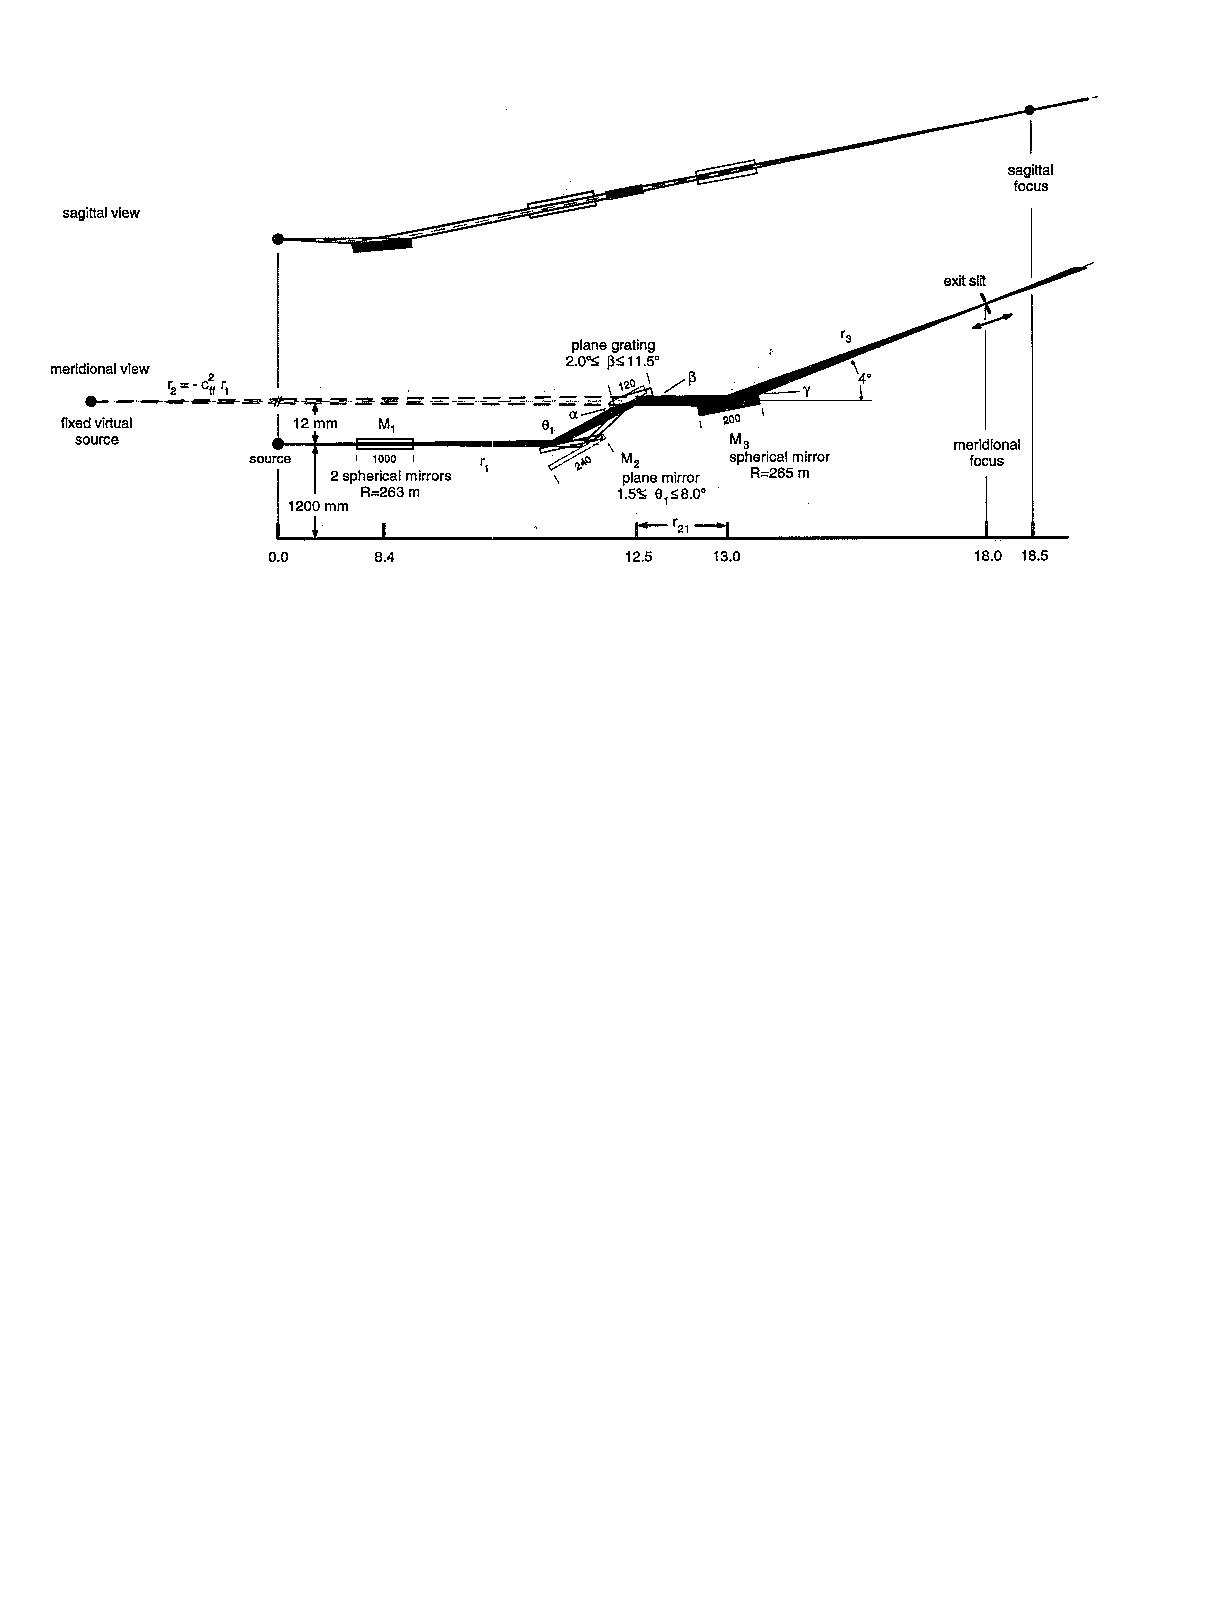
\includegraphics[scale=1]{../data/Chapter1/1c_monoExample/1c_bessy_HE-PGM-3.pdf} 
%   \caption{The Petersen Plane Grating Monochromator, as implemented on the HE-PGM-3 beamline at BESSY.  In Ref. \cite{Pet95}, Petersen et. al. provide a good overview of monochromator focussing techniques, prior to the widespread adoption of VLS designs.  \textbf{Image from:} \cite{Pet95}.}
%   \label{1c}
%\end{figure}

\subsubsection{Spectrometers}
If the goal of a monochromator is to produce monochromatic light, the goal of a spectrometer is to produce a \emph{spectrum} -- ie: to resolve the frequency components that exist in an unknown light source and measure their relative intensity.  The device in Figure \ref{1b_mirrorSpectrometer} is identical to the monochromator shown in Figure \ref{1b_monochromator}, except that the exit slit has been replaced by an area-sensitive detector.  With the grating positioned so that an outgoing diffraction order (typically the 1st order, for best efficiency) lands on the detector, the angular dependence on wavelength puts short wavelengths onto the top of the detector, and long wavelengths onto the bottom of the detector.  The intensity profile recorded across the detector surface is a spectrum, although some mathematical correction will need to be done to calibrate the energy axis, by mapping detector positions to diffraction angles, and diffraction angles to energy using the grating equation.

The spectrometer in Figure \ref{1b_rowlandSpectrometer} is more representative of those used in soft x-ray applications, where the low initial levels of fluorescence from the sample and the poor reflectivity of mirrors make it desirable to eliminate as many optical components as possible.  Just like monochromators, spectrometers must focus light from the entrance slit -- or directly from the source, in the case of slit-less designs -- onto the detector.  This is accomplished by using spherical gratings and arranging the geometry to exploit the \emph{Rowland Circle} focussing condition discovered by Henry Rowland \cite[p.~169]{Pea97}, or again by using VLS gratings to alter the shape of the focal curve.  More information on spectrometer focussing can be found in the M.Sc. thesis by David Muir \cite{Mui06}.

Like monochromators, spectrometer designs usually offer switchable gratings with different line densities and coatings, optimized for different energy ranges as we show in Chapter 5 of my thesis draft.  Figure \ref{1d} shows a top and side view of the SXF endstation on Beamline 8.0.1 of the Advanced Light Source, a typical ``workhorse'' spectrometer, which balances moderate resolution with reasonable efficiency.  It uses four gratings with groove densities of 600, 1000, and 1500 lines/mm to cover the energy range from 70 to 1200 eV, and uses a 40 mm wide multi-channel plate detector with an effective spatial resolution between 40 and 80 um.  Figure \ref{1e} shows an image recorded by that detector, and the corresponding spectrum.

\begin{figure}[htbp] %  figure placement: here, top, bottom, or page
   \centering
   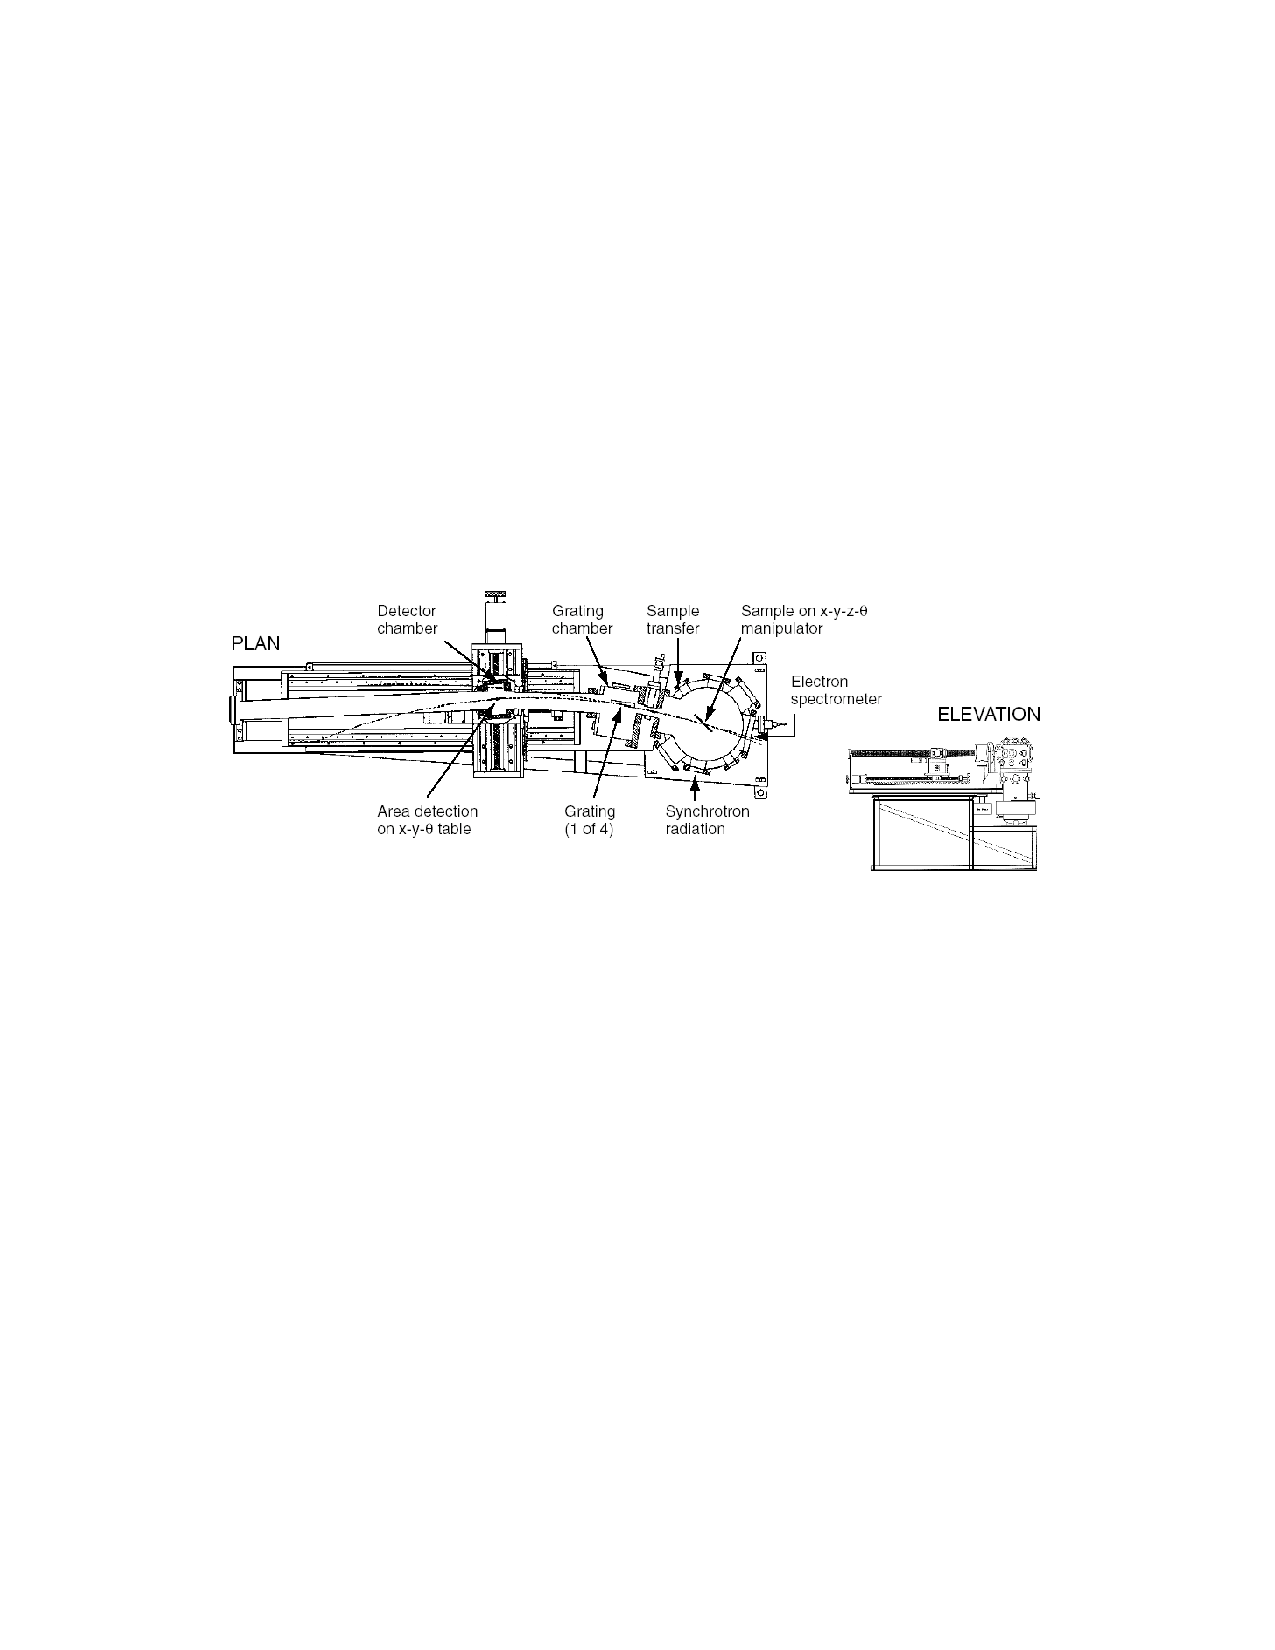
\includegraphics[scale=1.2]{../data/Chapter1/1d_spectrometerExample/1d_bl801SXF_2.pdf} 
   \caption{The SXF endstation spectrometer on Beamline 8.0.1 of the Advanced Light Source -- a typical ``workhorse'' spectrometer.  It uses spherical gratings in a Rowland Circle design; four gratings let users choose between higher resolution or higher efficiency at different energy ranges.  
   % TODO The resolving power of this machine is compared with other leading spectrometers in Figure \ref{4a}.  \textbf{Image from:} \cite{Jia95}
   }
   \label{1d}
\end{figure}

\begin{figure}htbp] %  figure placement: here, top, bottom, or page
   \centering
   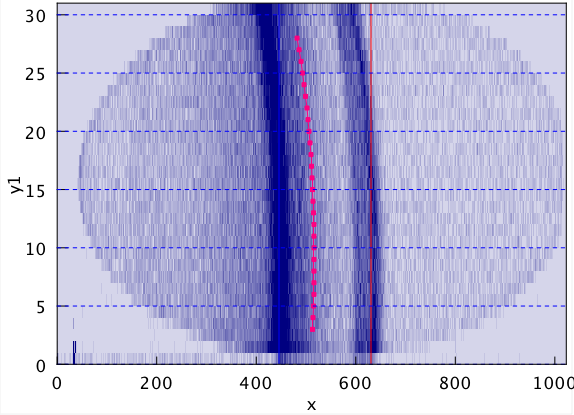
\includegraphics[height=2in]{../data/Chapter1/1e_spectrometerData/1e_image.png} 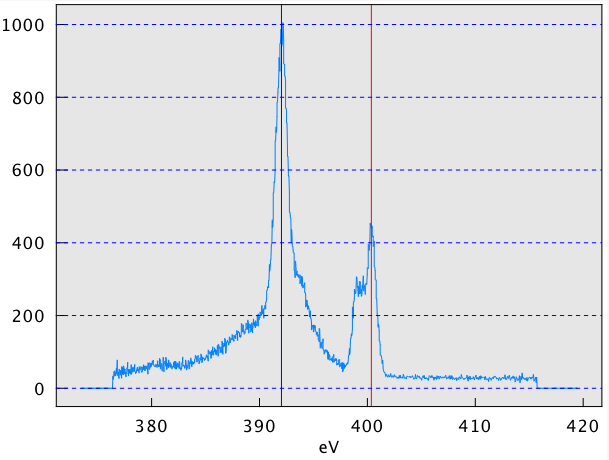
\includegraphics[height=2in]{../data/Chapter1/1e_spectrometerData/1e_spectrum.png}
   \caption{A detector image and corresponding spectrum produced by the SXF spectrometer in Figure \ref{1d}.  (This particular scan is of the nitrogen emission lines in nitrogen-doped zinc oxide.)  The curvature of the spherical gratings provides focussing in the dispersion direction ($x-$axis), but unfortunately produces a curved image in the perpendicular direction ($y-$axis).  This curvature is corrected by aligning rows along the red curve when the image is summed to produce the spectrum on the right.}
   \label{1e}
\end{figure}

\subsection{Goals for Soft X-ray Instruments}
\label{resolutionGoals}
In the design of both spectrometers and monochromators, there are two goals we have already mentioned that are important from the experimenter's perspective:
\begin{itemize}
\item The \textbf{resolution} is important in order to see details in spectra and probe new science.  On a soft x-ray beamline, the monochromator determines the resolution of an absorption scan, and the spectrometer determines the resolution of an emission scan.  Both are involved in the experimental resolution of RIXS studies.
\item The overall \textbf{efficiency} is important because it determines how much light is available, and indirectly how long it takes to generate enough photon interactions to record acceptable statistics.  At a minimum, the efficiency must be high enough to produce a signal above the background noise level of the detector.  Beyond this threshold, increases in efficiency make it faster to do experiments and let the user accomplish more science in their shift.
\end{itemize}

Since the probability of an excited atom decaying via fluorescence transitions is so low compared to other decay methods, the initial amount of light available in emission experiments is extremely low.  This is further compounded in experiments on doped or dilute samples, when trying to observe the emission lines of the dopant elements.  Finally, the entrance slit of a spectrometer can only capture a tiny geometric fraction of all photons out of the sample.  All of these reasons combine to make emission spectroscopy experiments extremely ``photon hungry'', which means that efficiency is especially critical here.

What makes these two goals challenging is that they are inherently in tension.  To see why, we consider as an example a simple emission spectrometer like the one shown again in Figure \ref{1f}.

\begin{figure}[htbp] %  figure placement: here, top, bottom, or page
   \centering
   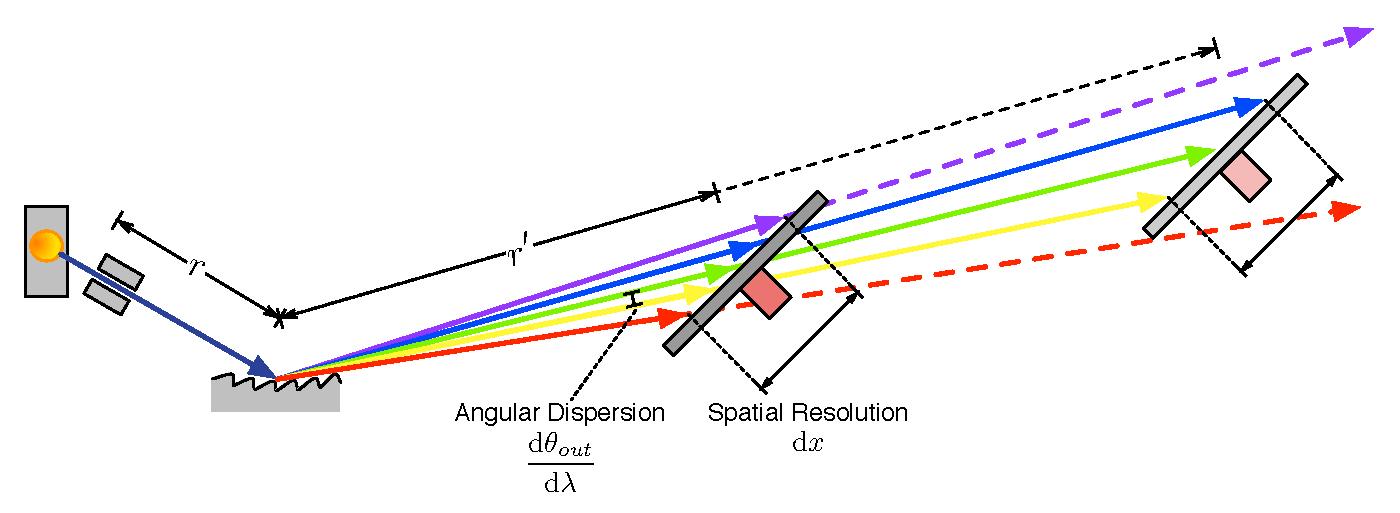
\includegraphics[scale=0.6]{../data/Chapter1/1f_spectrometerResolution/1f_2.pdf} 
   \caption{The detector has an effective spatial resolution $\mathrm{d}x$ which is the minimum distance required to resolve two adjacent incident rays.  Except for the $n=0$ order, the grating produces an angular dispersion $\mathrm{d}\theta_{2,n}/\mathrm{d}\lambda$, which is the angular separation between infinitesmally-adjacent wavelengths.  To increase the spacing between adjacent wavelengths on the detector, we can either increase the grating-detector distance $r^\prime$, or increase the angular dispersion. }
   \label{1f}
\end{figure}
               
The immediate result of a spectroscopy experiment is the image produced along the detector surface.  For all detectors -- be they photographic film, multi-channel plate detectors, or CCDs -- there is an \emph{effective spatial resolution}: the minimum distance along the detector that is required for two adjacent rays to be distinguished.  For a given detector, if you wanted to increase the \emph{energy resolution}, you would want to either 
\begin{enumerate}
\item increase the angular dispersion of the grating -- thereby increasing the angular separation between adjacent wavelengths, or 
\item you would want to put the detector a long way from the grating, so that over distance the angular dispersion creates a large spatial separation between adjacent wavelengths.
%TODO \footnote{This is why currently the world's two highest-resolution emission endstations use 10 meter- and 50 meter-long spectrometers; see section TODO.}
\end{enumerate}

Both of these solutions inherently reduce the \emph{geometric efficiency} of the spectrometer: the fraction of all photons captured by the detector assuming perfect mirror and grating efficiency.  In the dispersion direction (or \emph{meridional} direction, vertical in Figure \ref{1f}), the detector will now only capture photons from a smaller energy range; the corresponding reduction in light gathered is an unavoidable tradeoff no matter what scheme is used to increase  resolution.  However, the second method -- increasing the distance from the grating to the detector --  reduces the solid angle captured by the detector also in the perpendicular direction (or \emph{saggital} direction, out of the page), further decreasing the geometric efficiency to an extent which depends on the nature of focussing in that direction.\footnote{A complete analysis of focussing criteria would show that, at least for Rowland Circle spectrometers, increasing the source-grating distance requires an increase in both the entrance slit-grating distance, \emph{and} an increase in the grating radius; both of these actions further decrease the geometric efficiency, possibly as as function of the cube of the distance.  One could compensate by using larger gratings, but the maximum grating size must be limited to manage spherical aberrations; see Ref. \cite[p.~98]{Mui06}.}  The only way to increase resolution with only the minimum essential reduction in geometric efficiency is by using the first method: increasing the grating's angular dispersion.  By differentiating the grating equation (\ref{gratingEquation}) with respect to wavelength (holding the incident angle $\theta_{2}$ constant):
\begin{eqnarray}
\frac{n\lambda}{d} &=& \sin\theta_{2,n} - \sin\theta_{2} \\
\frac{n}{d} &=& \cos \theta_{2,n} \frac{\dif \theta_{2,n}}{\dif \lambda} \\
\frac{\dif \theta_{2,n}}{\dif \lambda} &=& \frac{n}{d\, \cos \theta_{2,n}}
\label{angularDispersionEqn}
\end{eqnarray}
we derive an expression for the angular dispersion; it is clear that to create more dispersion, we can either increase the groove density (decrease the groove spacing $d$), or use a higher diffraction order $n$.  Unfortunately, as will be shown in Chapter 5 of my thesis draft, both of these actions substantially reduce the \emph{grating efficiency}.  As an additional challenge, we can see that the dispersion will be reduced for higher energies, which leave the grating at more normal angles, creating a larger $\cos \theta_{2,n}$.

No matter which method is used, resolution and overall efficiency are in conflict.  Whether it is a hit to the grating or to the geometry, increasing the resolution demands a reduction in efficiency and vice-versa, the cleverness of the beamline designer being measured in his or her ability to negotiate this compromise.

While this example examined resolution as seen by a spectrometer detector, the same unfortunate principles apply to monochromators as well.

\subsection{Challenges of Soft X-ray Applications}
\label{challengesSXS}
All grating spectrometers, regardless of their wavelength range, are subject to the unavoidable tradeoff between resolution and efficiency.  However, the nature of soft x-rays adds an additional set of challenges within this regime, which combine to make efficiency even more important.

\subsubsection{UHV Compatibility}
Because the energy of soft x-ray photons matches the energy of core level electron transitions in all light elements, they are readily absorbed in matter over very short distances.  (Just passing through 1 mm of nitrogen at atmospheric pressure is enough to attenuate a 200 eV beam by 63 percent!)  For starters, this means that all SXS experiments must be done under \emph{ultra-high vacuum} (UHV) conditions, where the beam path has been evacuated of air and other contaminants, ideally to a pressure lower than $10^{-8}$ torr.  This is accomplished by using vacuum chambers and sealed beam pipes, pumped down using turbo-molecular pumps, ion pumps, and/or cryogenic pumps.  At these low pressures, most common materials would ``out-gas'', boiling off contaminants into the vacuum environment.  As a result, chambers and instrumentation must be built using a restricted set of UHV-compatible materials (certain grades of stainless steel and aluminum, copper, gold, and some special ceramics and high-temperature thermoplastics).  Anything that comes into contact with the vacuum environment must be carefully cleaned prior to assembly, and it is often necessary to ``bake out'' the chambers by heating them to temporarily raise the vapour pressure while pumping in order to remove water and other contaminants adsorbed to the inside surfaces before eventually attaining UHV levels.

For the experimenter, UHV requirements also apply to samples.  Liquid samples and non-UHV-compatible samples must be carefully enclosed and sealed behind thin windows to let the beam in. (Beryllium is often used in this application, due to its strength and relatively low absorption).  Loading samples into the vacuum chamber must be done through an airlock, and remote actuators are required to adjust the sample position and the position of optical elements.

\subsubsection{Low Reflectivity and Grazing Incidence}
Beamline designers face a more significant challenge when choosing optical elements.  The easy absorption of soft x-rays means that mirror and grating surfaces have extremely low reflectivity at these wavelengths -- at least at normal incidence.  For visible light, the reflectivity of a polished aluminum surface approaches 90\%; at 200eV, the reflectivity of the same surface is less than 0.005\% \cite{CXR11}.

Two approaches are necessary to work around this challenge.  Optical coatings need to be selected to avoid absorption edges in the region of interest.  For example, carbon and nickel have relatively high peak reflectivities 
% TODO (Figure \ref{3g}), 
but very strong absorption features at 284 eV and 853 eV respectively; these coatings would only be appropriate for optical elements used within a narrow wavelength range away from those edges.  In many-electron materials like gold and platinum, the most pronounced core-level absorption edges occur outside the soft x-ray region, and as result they have acceptable reflectivity over a wide bandwidth.\footnote{Gold and platinum do have absorption edges in the soft x-ray range, but these correspond to outer shell electrons (for example, gold 4s electrons bound at 802 eV) instead of core-level electrons. The outer electrons see shielding by the inner ones, and therefore have a lower transition probability.}

\label{TER-intro}
Second, mirrors and gratings need to be aligned and used at \emph{grazing incidence} -- i.e., with the incident light striking them at glancing angles just a few degrees from parallel to their surface.  At soft x-ray wavelengths, most materials have a refractive index with a real part \emph{less than} one; the phase velocity of light is actually \emph{faster} than it would be in a vacuum.  This allows us to exploit the phenomenon of total internal reflection (TIR), except in this case it becomes a \emph{total external reflection}, since the refractive index is higher in the grating material than it is in the vacuum above it.  Just as with conventional TIR in glass and air, we can calculate a critical angle above which total external reflection will occur.  
% TODO (see Section \ref{TER} of my thesis draft)
For most metals, this turns out to be around 83 to 85 degrees from the surface normal.

\section{REIXS spectrometer project}
This thesis -- and its motivation to establish a better understanding of diffraction grating efficiency -- emerged from a primary engineering goal: to design and build a world-class emission spectrometer for the REIXS beamline at the Canadian Light Source.  The REIXS (\emph{Resonant Elastic and Inelastic X-ray Scattering}) beamline is optimized for material science experiments; it offers an elliptically-polarizing undulator to produce a high brightness beam of soft x-ray photons, and a high-resolution monochromator with a flux of $\sim10^{13}$ photons/second and a resolving power greater than 5000.  The beamline has room for two endstations; our task was to build the emission spectrometer, which will be used for inelastic scattering experiments, while a team from the University of British Columbia built the second endstation used for elastic scattering measurements.

In Chapter 5 of my thesis draft, I describe the design process and the resulting optical design of the spectrometer.  Used in combination with the work of David Muir on spectrometer resolution \cite{Mui06}, the ability to model grating efficiencies allowed us to optimize the design for an intelligent compromise between these two competing goals.  In the process, we discovered an efficiency peak in the 3rd order -- typically assumed to be unusable -- that prompted us to create an innovative design capable of reaching much higher resolution than would otherwise be possible given the space constraints of the beamline.

%Figure \ref{1g} is a picture of the REIXS spectrometer as built, in August 2011.

%(TODO picture)

 \section{Summary: Why Grating Efficiency Matters}
 Figure \ref{1h} lists a variety of soft x-ray spectroscopy techniques, and shows the number of gratings in the beam path to the detector for each.  Of these techniques, those in \emph{italic text} are possible on the REIXS beamline; the remaining are possible on other beamlines at the CLS.  For all of these techniques, the ability to create more efficient gratings would increase the speed of experiments, improve the quality of data, and increase the minimum concentration of samples that can be feasibly studied.
 
 Conversely, during the design phase of these kinds of instruments, the unavoidable tradeoff between resolution and efficiency implies that accurate predictions of the grating efficiency could ironically be used improve \emph{resolution}: by deliberately sacrificing efficiency, designers could push their resolving power to the limit once the efficiency is known to be ``good enough''.
 
 \begin{figure}[htbp] %  figure placement: here, top, bottom, or page
   \centering
   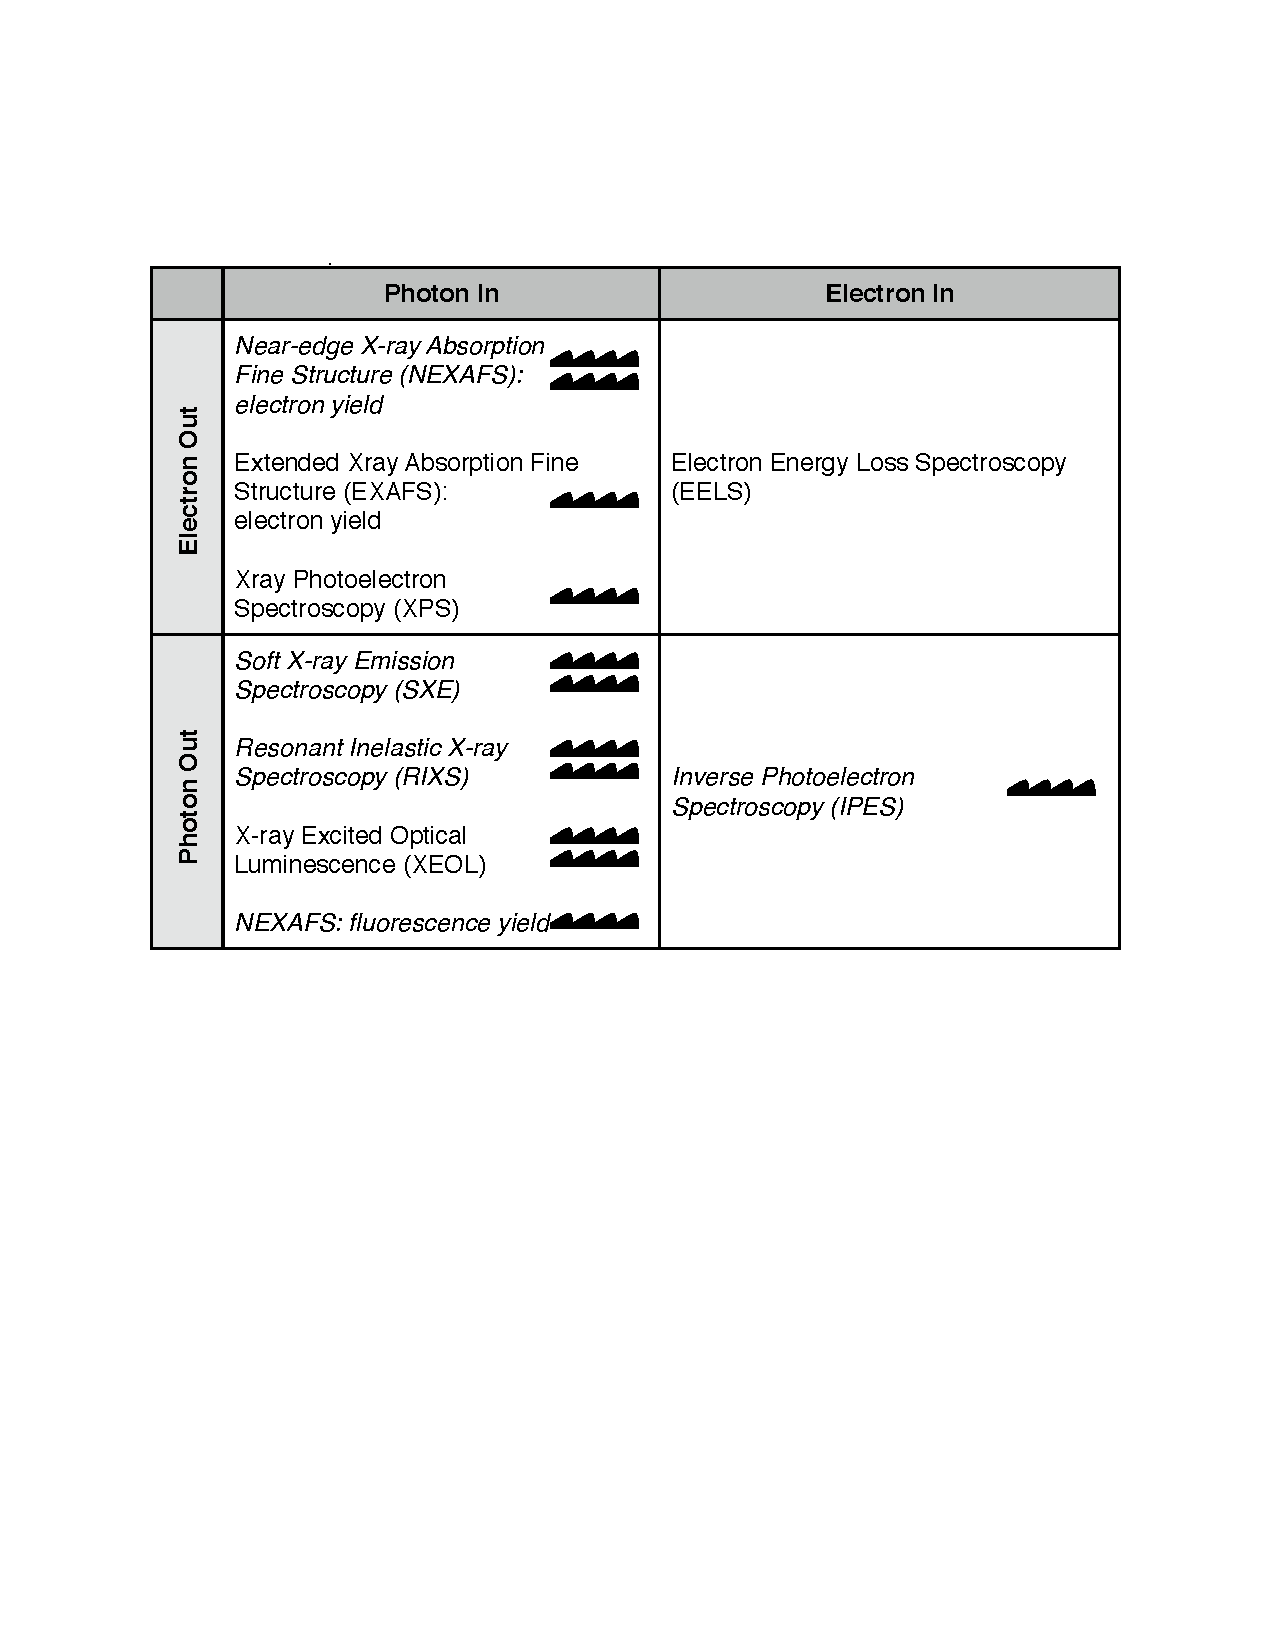
\includegraphics[scale=0.8]{../data/Chapter1/1h_techniques/1h.pdf} 
   \caption{A variety of soft x-ray spectroscopy techniques, and the number of gratings required in the beam path to accomplish each one.  Of these techniques, those in \emph{italic text} are possible on the REIXS beamline using the emission spectrometer endstation.  For all these techniques -- and particularly those using two gratings -- more efficient gratings would increase the speed of experiments, improve the quality of data, and increase the minimum concentration of samples that can be feasibly studied.}
   \label{1h}
\end{figure}
 